\documentclass{article}
\usepackage{graphicx}
\usepackage[T1]{fontenc}
\usepackage{amsmath}
\usepackage{float}
\usepackage{enumitem}

\title{Zadanie projektowe 1}
\author{Julian Jaroszyński}
\date{listopad 2023}
\begin{document}

\maketitle
\tableofcontents

\newpage
\section*{Wstęp}
	Jujubee S.A. to studio deweloperskie zajmujące
	się tworzeniem gier wideo, które ma swoim koncie
	takie tytuły jak: „FLASHOUT 3D”, „Suspect in
	Sight”, „Take Off – The Flight Simulator”,
	strategię czasu rzeczywistego „Realpolitiks”, grę
	przygodowo-dokumentalną „KURSK” oraz „Deep Diving
	Simulator”. Studio zostało założone przez byłych
	pracowników CD Projekt RED, Traveller’s Tales oraz
	Inifinite Dreams. Celem firmy jest tworzenie niesamowicie
	grywalnych i doskonale wyglądających gier na wszystkie
	istotne platformy sprzętowe, takie jak iOS (iPhone,
	iPod, iPad), Android, Mac, PC i konsole. Jujubee jest
	spółką notowaną na rynku NewConnect (JJB).
\newpage
\section{Kursy zamknięcia}
	Wykres przedstawiający kursy zamknięcia firmy Jujubee S.A. (jjb) wraz z histogramem
	\begin{figure}[H]
		\centering
		\renewcommand\figurename{Wykres}
		\includegraphics{cena_podczas_zamkniecia.jpg}
		\caption{kursy zamknięcia}
	\end{figure}
	\begin{figure}[H]
		\centering
		\renewcommand\figurename{Wykres}
		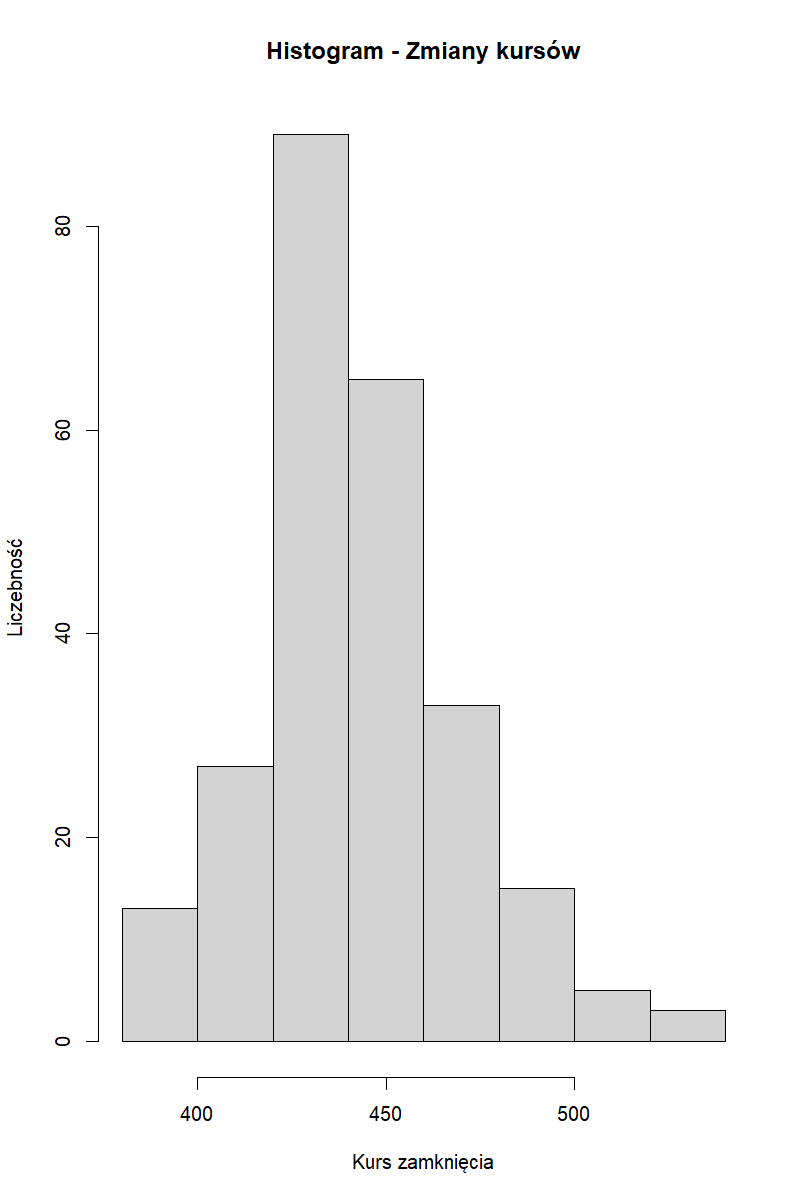
\includegraphics{histogram.jpg}
		\caption{histogram}
	\end{figure}
\newpage
\section{Statystyki opisowe}
	Jest to skośnść prawostronna (liczba jest dodatnia), oznacz to że jest
	dużo przypadków mniejszych od średniej, firma miała parę dużych kursów
	podbijających średnią;
	Jest to rozkład leptokurtyczny, oznacz to że wartości są skoncentrowane
	wokół śreniej oraz to że istnieje duża szansa na pojawienie się
	odstających obserwacji
	\begin{table}[h]
		\centering
		\renewcommand\tablename{Tabela}
		\begin{tabular}{|c|c|c|c|c|}
			\hline
			 & $\bar{x}$ & odch. st. & skośność & kurtoza \\
			\hline
			Akcja & 2.017201 & 0.5117912 & 1.319479 & 1.417186 \\
			\hline
		\end{tabular}
		\caption{statystyki opisowe}
		\label{tab:przyklad}
	\end{table}
\newpage
\section{Parametry rozkładów}
	Parametry trzech rozkładów
	\begin{table}[h]
		\renewcommand\tablename{Tabela}
		\centering
		\begin{tabular}{|c|c|c|}
			\hline
			& estymator & błąd \\
			\hline
			średnia & 2.0172008 & 0.03236826\\
			\hline
			sd & 0.5107625 & 0.02288742\\
			\hline
		\end{tabular}
		\caption{parametry rozkładu normalnego}
	\end{table}
	\begin{table}[h]
		\renewcommand\tablename{Tabela}
		\centering
		\begin{tabular}{|c|c|c|}
			\hline
			& estymator & błąd \\
			\hline
			średnia & 0.6736043 & 0.01461544 \\
			\hline
			sdlog & 0.2306277 & 0.01033380 \\
			\hline
		\end{tabular}
		\caption{parametry rozkładów log-normalnego}
	\end{table}
	\begin{table}[h]
		\renewcommand\tablename{Tabela}
		\centering
		\begin{tabular}{|c|c|c|}
			\hline
			& estymator & błąd \\
			\hline
			kształt & 17.954308  & 1.5943798 \\
			\hline
			rate & 8.900479  & 0.8015123 \\
			\hline
		\end{tabular}
		\caption{parametry rozkładów gamma}
	\end{table}
\newpage
\section{Wykresy diagnostyczne}
	na podstawie tych 4 wykresów można wywnioskować że wykres
	lnorm jest najlepiej opisujący kursy zamknięcia, ale aby to
	dokładnie stwierdzić trzeba wykonać analizę statystyk KS,
	CM i AD oraz kryteriów informacyjnych AIC i BIC
	\begin{figure}[H]
		\centering
		\renewcommand\figurename{Wykres}
		\includegraphics[width=1.25\textwidth]{comp.jpg}
		\caption{kursy zamknięcia}
	\end{figure}
\newpage
	\subsection{KS, CM, AD}
		Analiza dopasowania rozkładów za pomocą
		testów Kolmogorova-Smirnova, Cramera-von Misesa i
		Andersona-Darlinga pokazuje, że dla rozkładu normalnego
		(norm), log-normalnego (lnorm) i rozkładu gamma (gamma)
		wartości statystyk są odpowiednio 0.1465, 0.0946 i
		0.1122 dla testu Kolmogorova-Smirnova, 1.5942, 0.5890
		i 0.8612 dla testu Cramera-von Misesa, oraz 10.0248,
		4.1675 i 5.7877 dla testu Andersona-Darlinga.
		\begin{table}[h]
			\renewcommand\tablename{Tabela}
			\centering
			\begin{tabular}{|c|c|c|c|}
				\hline
				& norm & lnorm & gamma \\
				\hline
				Kolmogorov-Smirnov statistic & 0.1464534 & 0.09463034 & 0.1121969 \\
				\hline
				Cramer-von Mises statistic & 1.5941731 & 0.58899369 & 0.8611976 \\
				\hline
				Anderson-Darling statistic & 10.0247605 & 4.16749359 & 5.7876581 \\
				\hline
			\end{tabular}
			\caption{Goodness-of-fit statistics}
		\end{table}
	\subsection{AIC, BIC}
		Porównanie kryteriów doboru modelu, takich jak Akaike's
		Information Criterion (AIC) i Bayesian Information
		Criterion (BIC), wskazuje, że dla rozkładu normalnego
		(norm), log-normalnego (lnorm) i rozkładu gamma (gamma)
		wartości wynoszą odpowiednio 376.0498, 315.5450 i
		331.6349 dla AIC, oraz 383.0847, 322.5800 i 338.6698
		dla BIC.
		\begin{table}[h]
			\renewcommand\tablename{Tabela}
			\centering
			\begin{tabular}{|c|c|c|c|}
				\hline
				& norm & lnorm & gamma \\
				\hline
				Akaike's Information Criterion & 376.0498 & 315.545 & 331.6349 \\
				\hline
				Bayesian Information Criterion & 383.0847 & 322.580 & 338.6698 \\
				\hline
			\end{tabular}
			\caption{Goodness-of-fit criteria}
		\end{table}
\newpage
\section{Testowanie hipotezy}
	Do przetestowania hipotezy został użyty sposób Kolmogorova-Smirnova
	(KS), którego wynikiem jest: 0.3202. Ta wartość jest większa
	niż 0.05, przez co można odrzucić kontr hipotezę
	\begin{figure}[H]
		\centering
		\renewcommand\figurename{Wykres}
		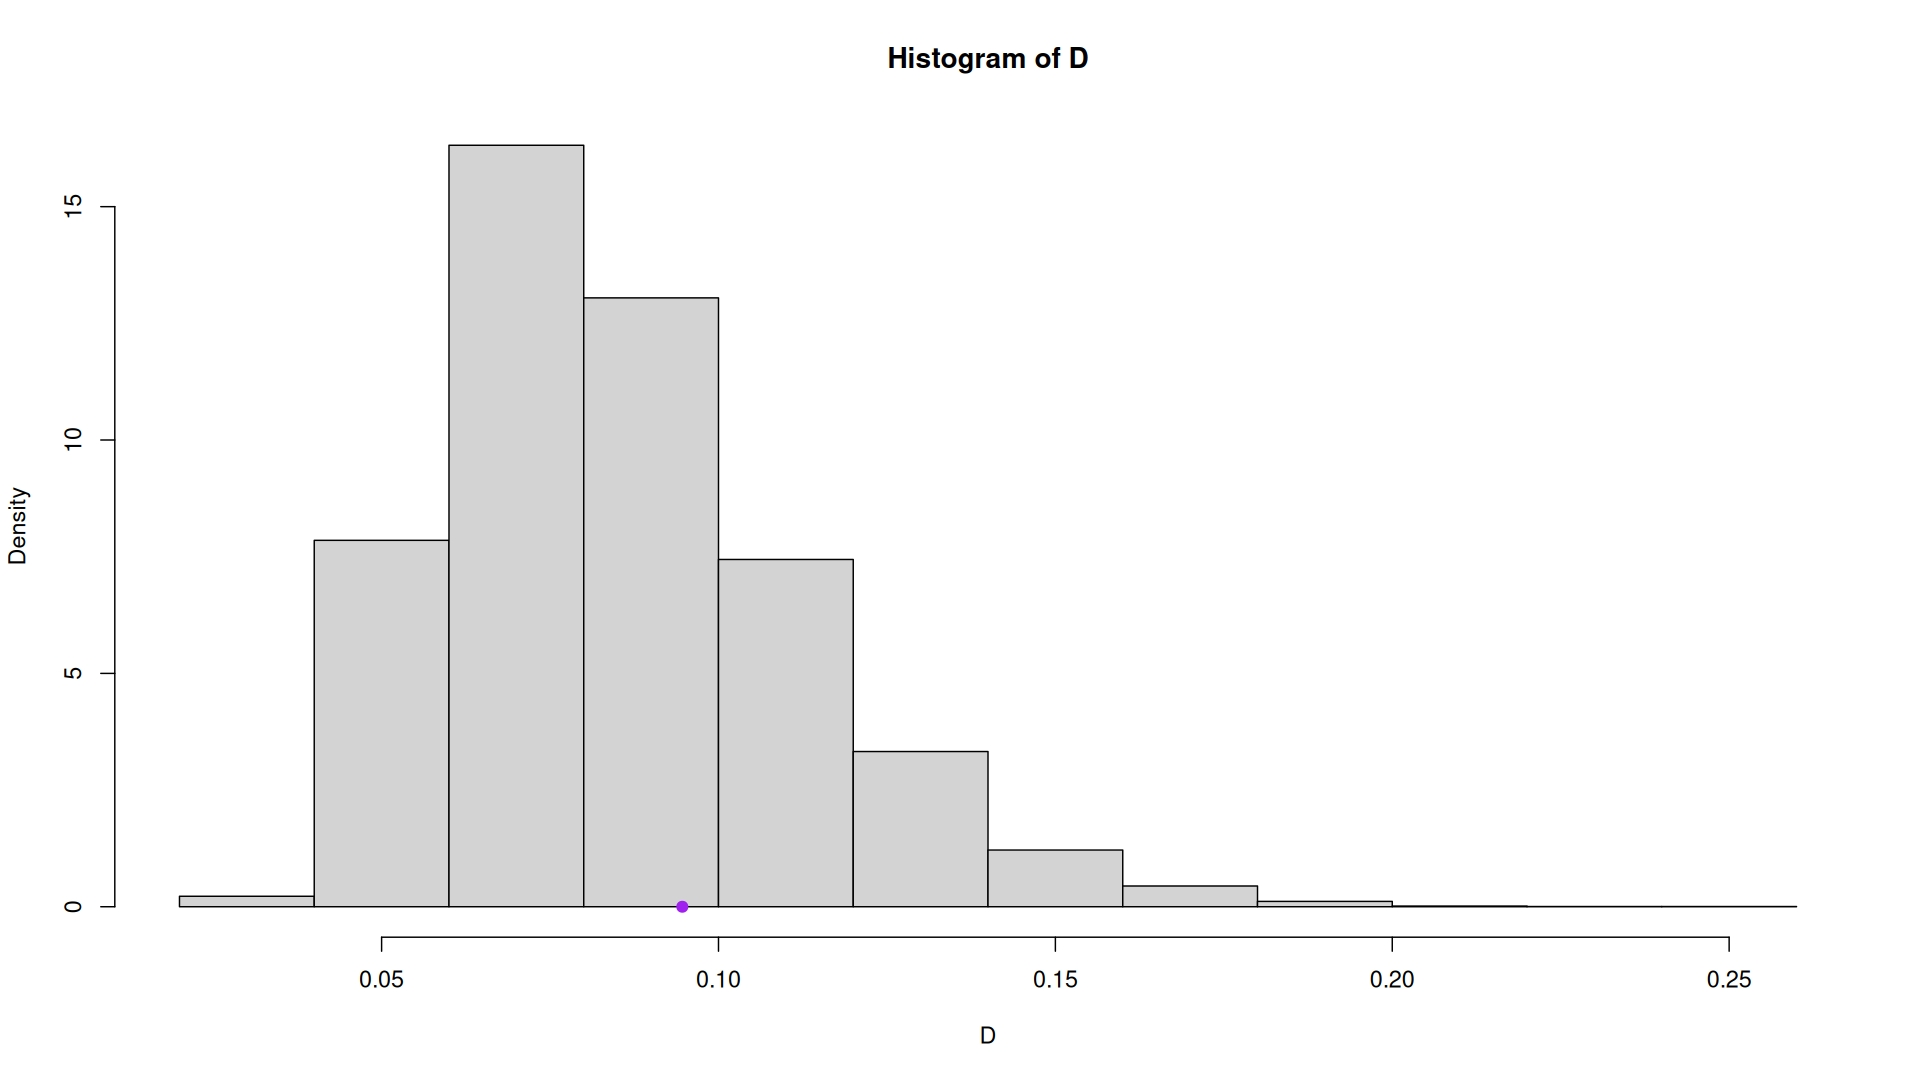
\includegraphics[width=1.25\textwidth]{hist2.jpg}
		\caption{histogram metody ks}
	\end{figure}

\end{document}
